% Reviewer 1 responses

\begin{point}
Jablonka et al give a sweeping, well-structured review on the promise of general-purpose models for the chemical sciences. I really like the balance of conceptual clarity and technical depth throughout the article, particularly in the figures that illustrate model workflows and representative examples. In my opinion, it does a great job covering multiple aspects of the GPM pipeline and I think this will be a nice contribution to the field. Overall I enjoy reading it and think it can be accepted with some minor revisions.
\end{point}

\begin{reply}
We sincerely appreciate the reviewer's positive feedback on our manuscript's contribution.
\end{reply}

\begin{point}
The article swings between LLMs and broader GPMs a bit inconsistently. Sometimes it reads as if the topic is ``large language models for chemistry'', and other times it zooms out to cover the broader general-purpose model landscape, including other architectures. I think the introduction could be clearer in stating exactly what is being covered, if over 80\% is for LLMs (or transformer-based foundation models), I think some modifications may be needed for title and abstract. Otherwise I feel somehow hard to get a sense of the entire field of GPM in Chemistry (and indeed this is a big scope). A one-sentence thesis and consistent reminders throughout the review would help readers track the core argument.
\end{point}

\begin{reply}
\label{reply:gpm_definition}
 To provide clearer direction, we have now introduced a new table (see \Cref{tab:gpm}) early in the paper that explicitly defines \glspl{gpm} and distinguishes them from other model types (domain-specific foundation models and specialized chemistry pipelines). This table provides concrete examples and clearly contrasts \glspl{gpm} with domain-specific foundation models (e.g., AlphaFold,\autocite{AlphaFold2021} ESM,\autocite{lin2022language} MACE-MP-0\autocite{batatia2023foundation}) and specialized chemistry pipelines (e.g., QSPR models, graph-based reaction predictors).

\begin{table}[H]
    \centering
    \caption{\textbf{Illustrative examples of GPMs, domain‑specific foundation models, and specialized chemistry ML pipelines}. The table depicts the definition of \gls{gpm} with examples for such models, as well as comparisons with domain-specific models and chemistry pipelines. Note that a \gls{gpm} does not necessarily output text.}
    \label{tab:gpm}
    \begin{tabularx}{\linewidth}{@{}p{0.22\linewidth} p{0.42\linewidth} X@{}}
        \toprule
        \textbf{Category} & \textbf{Typical Characteristics} & \textbf{Representative Examples} \\
        \midrule
        \addlinespace[0.3em]
        
        \glspl{gpm} &
        Pre‑trained on a large heterogeneous corpus spanning multiple modalities. Supports zero/few‑shot generalization and can be fine‑tuned for diverse chemistry tasks. Capable of autonomous agent behavior, including planning and execution. &
        \textbf{Autoregressive:} GPT‑4,\autocite{openai2023gpt04} LLaMA,\autocite{grattafiori2024llama} Galactica\autocite{taylor2022galactica}
        
        \textbf{Diffusion-based:} Gemini Diffusion,\autocite{deepmind_geminidiffusion_2025} Inception Mercury\autocite{inceptionlabs2025mercury0}
        
        \textbf{Other:} Mamba-based\autocite{gu2023mamba0} models \\
        
        \addlinespace[0.8em]
        \midrule
        \addlinespace[0.3em]
        
        Domain‑Specific Foundation Models &
        Trained on curated, domain‑specific datasets (e.g., protein structures, crystal structures). Achieve state‑of‑the‑art performance in narrow task sets, but are typically not multimodal or generalizable to unrelated chemistry problems. &
        AlphaFold,\autocite{AlphaFold2021} ESM,\autocite{lin2022language} MACE-MP-0\autocite{batatia2023foundation}, MatterSim\autocite{yang2024mattersim}, MolecularTransformer\autocite{schwaller2019molecular} \\
        
        \addlinespace[0.8em]
        \midrule
        \addlinespace[0.3em]
        
        Specialized Chemistry Pipelines &
        Domain‑specific models combined with rule‑based or symbolic components. Often rely on hand‑crafted descriptors with limited transferability beyond the target task. &
        Graph‑based reaction outcome predictors,  \gls{qspr} models using Morgan fingerprints, \gls{gpr} on \gls{nmr} shifts \\
        
        \addlinespace[0.3em]
        \bottomrule
    \end{tabularx}
\end{table}

Additionally, we added the following text in section 1, and we reviewed the usage of \gls{gpm} and \gls{llm} throughout the manuscript to ensure that they are correctly applied according to this definition. 
\begin{quote}
A \gls{gpm} is a model that has been pre‑trained on a broad, heterogeneous corpus spanning multiple data modalities (text, images, graphs) or representations (e.g., common names, 3D coordinates, molecular images).
It can be applied to a wide spectrum of downstream tasks that differ in objective (classification, regression, generation, reasoning), input format, and domain---ranging from natural‑language processing to chemistry and vision---with little or no task‑specific fine‑tuning.
A \gls{gpm} supports zero‑shot, few‑shot, or transfer learning and can serve as the core component of autonomous agents.
\end{quote}

In addition, we also updated the title of the manuscript to now read \enquote{General-Purpose Models for the Chemical Sciences:
LLMs and Beyond}.
\end{reply}

\begin{point}
Along those lines, Section 2 and 3 are strong technically, but could benefit from reiterating why these details matter specifically for chemistry-focused GPMs (instead of looking like a general background section for ML in Chemistry review paper). There's a lot on tokenization, embeddings, and architectures (which I appreciate), but the chemical intuition sometimes gets lost. While figures do include some chemistry example, some synthetic chemists without too much background may find confusing. I'd suggest adding short framing sentences to keep readers anchored in chemistry even as the model mechanics get dense.
\end{point}

\begin{reply}
\label{reply:example_boxes}
To address this concern, we have now integrated \enquote{example boxes} throughout our article, especially in section 3. We hope these dedicated boxes walk readers through key concepts with chemistry-specific examples, helping to maintain the connection to chemistry even as we discuss technical details about models' architectures. Below is one such example box we added to illustrate agent-based reasoning for chemical structure elucidation.

\begin{examplebox}[label={example:structure_eluc}]{Agent-based reasoning for chemical structure elucidation} 
\textbf{User Query:} \enquote{Identify this unknown white solid organic compound from analytical data.}

\textbf{Agent Reasoning Cycle:}
\begin{enumerate}
\item \textbf{THINK:} \enquote{Unknown white solid. Need to analyze all spectra systematically.}
\item \textbf{ACT:} Analyze \texttt{IR} spectrum tool $\rightarrow$ Output peak data (\SIrange{3000}{3500}{\per\cm} broad, \SI{1680}{\per\cm} sharp, \SI{1600}{\per\cm}, \SI{1500}{\per\cm}).
\item \textbf{ACT:} Analyze \texttt{MS} tool $\rightarrow$ Output peak data (\texttt{Top 3 peaks (135.0, 26.48)}, \texttt{(106.9, 0.43)}, \texttt{(120.4, 0.31)}).
\item \textbf{OBSERVE:} \enquote{Broad \texttt{O-H} stretch suggests carboxylic acid. Sharp \texttt{C=O} at \texttt{1680} indicates aromatic carboxylic acid. Aromatic \texttt{C=C} stretches confirm benzene ring, and \texttt{MS} tool suggests molecular formula \ce{C8H8O2}.}
\item \textbf{THINK:} \enquote{Aromatic carboxylic acid with \ce{C8H8O2}... probably substituted benzoic acid. Need to determine substitution pattern.}
\item \textbf{ACT:} Run \ce{^1H} \texttt{NMR} integration tool $\rightarrow$ Input chemical shifts (\texttt{7.8 ppm} doublet, \texttt{7.3 ppm} doublet, \texttt{2.4 ppm} singlet, \texttt{12.1 ppm} broad).
\item \textbf{OBSERVE:} \enquote{Two aromatic doublets suggest para-disubstitution. Singlet at \texttt{2.4 ppm} integrates for \texttt{3H} --- likely \ce{CH3}. Broad peak at \texttt{12.1 ppm} confirms \ce{COOH}.}
\item \textbf{THINK:} \enquote{Para-disubstituted benzene with \ce{CH3} and \ce{COOH} groups. Could be \textit{p}-toluic acid.}
\item \textbf{ACT:} Search chemical database for \enquote{\texttt{para-methylbenzoic acid}}.
\item \textbf{OBSERVE:} \enquote{\texttt{4-methylbenzoic acid} (\textit{p}-toluic acid) matches: \ce{C8H8O2}, \texttt{mp} \SI{180}{\degree C}.}
\item \textbf{ACT:} Run structure validation tool $\rightarrow$ Compare predicted vs. observed spectra.
\item \textbf{OBSERVE:} \enquote{Predicted \ce{^1H} \texttt{NMR}: $\delta$  \texttt{7.9 (d, 2H)}, \texttt{7.2 (d, 2H)}, \texttt{2.4 (s, 3H)}, \texttt{12.0 (br, 1H)}. Perfect match!}
\item \textbf{ACT:} Cross-reference \texttt{MS} fragmentation pattern tool.
\item \textbf{OBSERVE:} \enquote{Base peak at \texttt{m/z 91} (tropylium ion, loss of \ce{COOH}), molecular ion at \texttt{136}. Consistent with \textit{p}-toluic acid fragmentation.}
\end{enumerate}


\textbf{RESULT:} Structure confirmed as \texttt{4-methylbenzoic acid}. All spectroscopic evidence supports this assignment.

The agent systematically combines \texttt{IR}, \texttt{NMR}, and \texttt{MS} data with database searching to solve a realistic structure determination challenge.
\end{examplebox}
\end{reply}

\begin{point}
Section 5.2, which lists existing GPMs for chemical sciences, feels very thin compared to the rest. This is a missed opportunity to give readers a map of the landscape. Many of the examples are mentioned quickly but not deeply described. I think most readers would want to know: which model should I try and why?
\end{point}

\begin{reply}
Following this suggestion, we have now expanded Section 5.2 to provide a more comprehensive map of the \gls{gpm} landscape for chemistry. We added a detailed table (see \Cref{tab:existing_gpms}) summarizing the key characteristics of available models---including their architecture (e.g., encoder-only, decoder-only, encoder-decoder, base model), training approach, representative tasks, and target systems (organic molecules, inorganic materials, proteins, etc.). This table helps readers understand the landscape of available \glspl{gpm} and make informed decisions about which model to use for their specific applications.
\begin{table}[H]
\centering
\setlength{\tabcolsep}{5pt}
\renewcommand{\arraystretch}{1.3}
\setlength{\extrarowheight}{0.3ex}
\caption{\textbf{Non-comprehensive list of existing \glspl{gpm} in chemical sciences.} Most current models are trained on a mixture of general and domain-specific corpora. Models are sorted by the order they appear in the main text.}
\label{tab:existing_gpms}
\footnotesize
\begin{tabularx}{\linewidth}{
  l
  >{\raggedright\arraybackslash}X
  >{\raggedright\arraybackslash}X
  >{\raggedright\arraybackslash}X
  >{\raggedright\arraybackslash}X
}
\toprule
\textbf{Model} & \textbf{Architecture} & \textbf{Training} & \textbf{Representative Tasks} & \textbf{Representative Systems} \\
\midrule
\modelname{DARWIN 1.5} \autocite{xie2025darwin} & decoder-only transformer (LLaMA) with 7B parameters & fine-tuning on \glspl{qa}; multi-task fine-tuning on language-interfaced classification and regression tasks &  materials property prediction from natural language prompts & inorganic materials \\
\addlinespace[2.5pt]
\modelname{ChemLLM} \autocite{zhang2024chemllm} & decoder-only transformer (InternLM2) with 7B parameters & instruction-tuning on template-based \glsps{qa} using \gls{sft} or \gls{dpo} & multi-topic chemistry \gls{qa} & organic molecules \& reactions \\
\addlinespace[2.5pt]
\modelname{nach0} \autocite{livne2024nach0} &
encoder–decoder transformer (T5) with 250M or 780M parameters &
pre-trained using \gls{ssl} on scientific literature and \gls{smiles} strings; instruction-tuned &
natural language to \gls{smiles}; small-molecule property prediction &
organic molecules \& reactions \\
\addlinespace[2.5pt]
% \modelname{MatBERT} \autocite{qu2023leveraging, wan2024tokens} &
% encoder-only transformer (BERT) with 110M parameters &
% masked language modeling pre-trained on materials literature; task-specific fine-tuning &
% create embeddings for property prediction &
% inorganic materials \\
% \addlinespace[2.5pt]
\modelname{LLaMat} \autocite{mishra2024foundational} &
decoder-only transformer (LLaMA) with 7B parameters &
continued pre-training on materials literature and crystallographic data &
materials information extraction; understanding and generating \glspl{cif} &
inorganic materials \\
\addlinespace[2.5pt]
\modelname{ChemDFM} \autocite{zhao2024chemdfm} &
decoder-only transformer (LLaMA) with 13B parameters &
pre-trained on 34B tokens from chemistry papers and textbooks; instruction-tuned with \gls{qa} and \gls{smiles} &
\gls{smiles} to text; molecule/reaction property prediction &
organic molecules \& reactions \\
\addlinespace[2.5pt]
\modelname{ether0} \autocite{narayanan2025training} &
decoder-only transformer (Mistral-Small) with 24B parameters; \gls{moe} &
\gls{sft} on reasoning traces, then \gls{rl} &
molecular editing; one-step retrosynthesis; reaction prediction &
organic molecules \& reactions \\
\bottomrule
\end{tabularx}
\end{table}

%We also expanded the discussion to include more details about each model, providing guidance on when to use specific models based on the task requirements and target chemical domain.
\end{reply}

\begin{point}
Section 5 and 6 make some strong claims about LLM-assisted discovery and autonomous science. But in practice, one risk can be most of these systems haven't gone beyond cherry-picking or recombining known ideas. One interesting thing author can consider (optional, totally up to them) is try to include a few concrete ``failure cases'' or borderline examples where the model output seems good on the surface but breaks under scrutiny. This could be framed as ``cautionary tales'' rather than critiques, which would add balance and practical value.
\end{point}

\begin{reply}
 We have now reviewed Sections 5 and 6, moderating the tone of the claims we make and adding explicit \textbf{Limitations} and \textbf{Open Challenges} subsections in each application section. For example in hypothesis generation section (section 5.4) we added

\begin{quote}
    \paragraph{Limitations}

Current \gls{llm}-driven systems lack the kind of creativity needed for paradigm-shifting hypotheses, tending to rearrange training data and retrieved content rather than propose genuinely new mechanisms. As a result, the evaluation of such outputs is also fragile, because using proxy metrics for \enquote{novelty} or \enquote{impact} that poorly track real scientific value can be deceiving. Finally, the problem’s open-ended nature makes systematic benchmarking ill-posed.

\end{quote}

 
 In addition, we added example boxes that focus and conceptualize some failure cases (see response \Cref{reply:planning_with_example})
 
\end{reply}

\begin{point}
Section 5 on planning and executing experiments are exciting, but a bit abstract. Are there concrete experimental workflows, for example, I know in past a few years some work in LLM + porous materials/polymer/ nanoparticle/ electrochemistry, that have been executed in real labs using these GPMs? If yes, even one well-described example would help readers from the experimental side understand what's actually possible. Also I think many examples the author mentioned are more on ``digital discovery'' side where the LLM were tested on real experimental dataset but not necessarily the verification are performed in real lab. So including some work with real lab verification (new discovery? not sure) may make a good balance and look convincing to experimentalist readers.
\end{point}

\begin{reply}
\label{reply:planning_with_example}
We have now added an illustrative example as a new figure (see \Cref{fig:planning_example}) in the planning section, demonstrating how an \gls{llm} can plan chemically to identify pairs of inorganic salts in solutions by decomposing the problem into sequences of experiments (acid/base tests). Importantly, this figure also highlights the limitations of current \gls{llm} planning capabilities by showing problematic steps in the plan with linked annotations explaining the errors. 

\begin{figure}[!htbp]
    \centering
        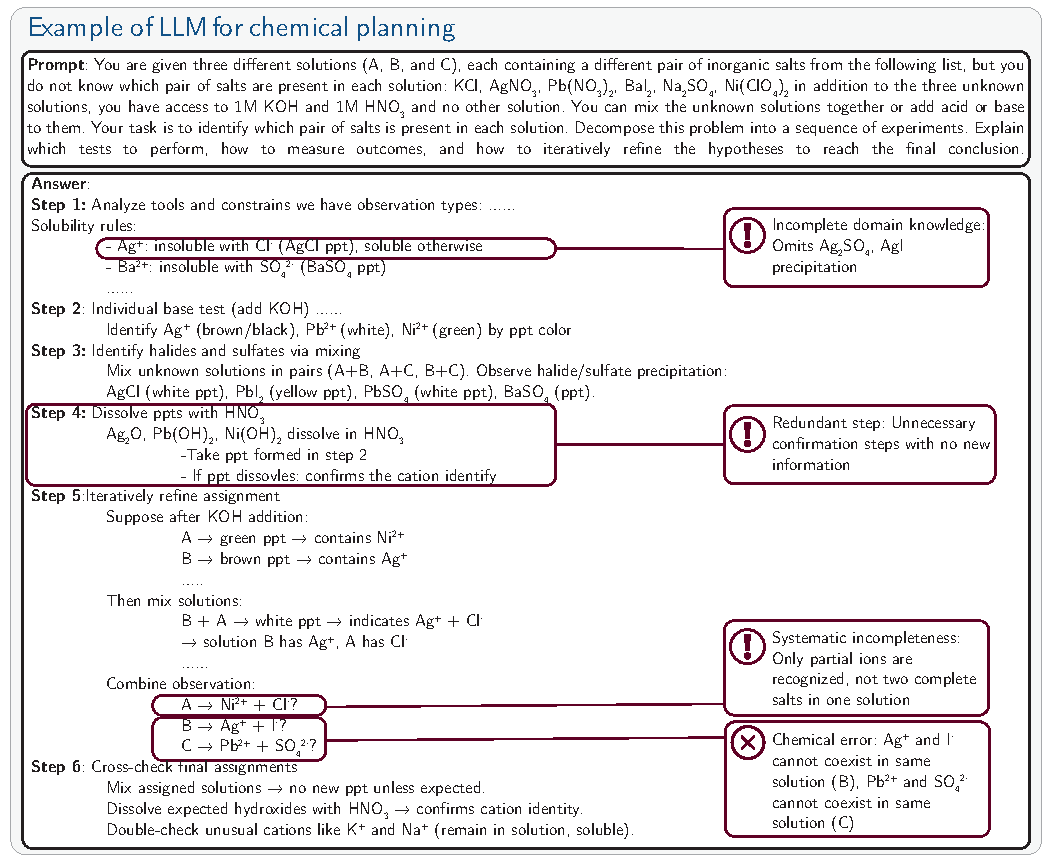
\includegraphics[width=1\textwidth]{figures/rescaled_figures/Chemrev_planning_example.pdf}
    \caption{\textbf{An example of using \gls{llm} for chemical planning to decompose problem}. \gls{llm} decomposes a chemical problem into sequential steps with detailed procedures. We manually evaluate the plan step by step, and highlight the problematic steps in text boxes, each linked to the corresponding reason. Plan generated by OpenAI GPT-5 (ChatGPT, web).
}
    \label{fig:planning_example}
\end{figure}

Additionally, in the experiment execution section, we now added concrete real-world examples (from \modelname{ChemCrow} and \modelname{ORGANA}) shown below, 

\begin{examplebox}[label={example:chemcrow_organa}]{Planning and executing experiments with \glspl{gpm}}

\textbf{ChemCrow:} When prompted with the task \enquote{Find and synthesize a thiourea organocatalyst which accelerates a Diels-Alder reaction}, \modelname{ChemCrow} sequentially queried tools to gather information and solve the task:

\par\vspace{0.5\baselineskip}

{\leftskip=2em \enquote{First, I need to find a thiourea organocatalyst that can accelerate the Diels-Alder reaction. I will perform a websearch to find a suitable catalyst.

\textbf{WebSearch tool:} Schreiner's thiourea catalyst

Now I will obtain the \gls{smiles}. 

\textbf{Name2Smiles tool:}

\texttt{FC(F)(F)c1cc(CN(=S)Nc2cc(C(F)(F)F)cc(C(F)(F)F)c2)cc(C(F)(F)F)c1}

I will plan a synthesis for Schreiner's thiourea catalyst. 

\textbf{SynthesisPlanner tool:} Detailed synthesis plan

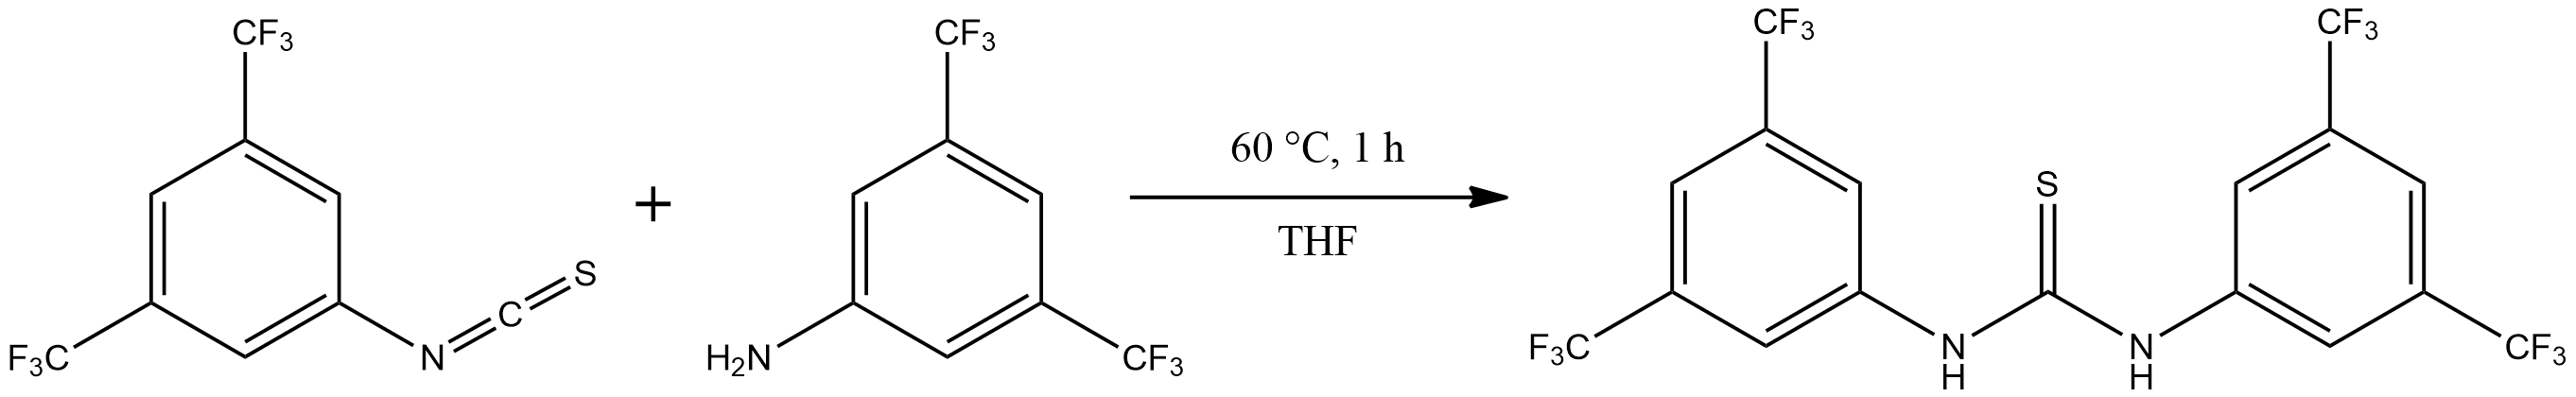
\includegraphics[width=0.8\textwidth]{figures/schreiner.png}

I will execute the synthesis.

\textbf{SynthesisExecuter tool:} Successful
synthesis.}

}

\par\vspace{0.5\baselineskip}

The agent proposed to synthesize the target molecule from the corresponding isothiocyanate and aniline derivatives and executed the synthesis on the RoboRXN platform. \autocite{roborxn} The product was confirmed using HPLC/MS: \texttt{m/z 501 [M+H]} calculated, found \texttt{m/z 501.02}.

\par\vspace{\baselineskip}

\textbf{ORGANA}: \modelname{ORGANA} interacts with chemists using \glspl{llm} to derive experiment goals and makes decisions with chemists in the loop to control robots and lab devices.
\begin{itemize}
    \item \textbf{Start-up:} Users give their intention \enquote{I want to create a Pourbaix plot of a quinone, Sodium Anthraquinone-1-sulfonate.}, and start interact with \modelname{ORGANA}:
    
    \modelname{ORGANA}: What is the setup of the lab environment? What hardware and reagents are present?
    
    User: I have a \SI{2}{\milli\molar} solution of the quinone......
    
    \modelname{ORGANA}: Can you provide an example of how to run the experiment? 
    
    User: Add \SI{2}{\milli\liter} of quinone......

    \modelname{ORGANA}: What is the expected outcome of the example experiment? 
    
    User: The pH of the solution is expected ......
    
    \modelname{ORGANA}: How many experiments are we planning to run in total? 
    
    User: 6
    
    \modelname{ORGANA}: Ok, thank you! I will start the experiment......

\end{itemize}

\end{examplebox}



\begin{examplebox}{Planning and executing experiments with \glspl{gpm} (ctd.)}

\begin{itemize}
    \item \textbf{Ambiguity and Uncertainty Mitigation:} 
    \modelname{ORGANA.Reasoner} evaluates whether experiment outcomes align with user expectations. If it can’t interpret the results, it alerts the user to check for environmental issues. The user provides feedback explaining the outcomes, which \modelname{ORGANA.Reasoner} then uses to refine its next plan:
    
    \enquote{I’m not sure what happened, but repeat the previous experiment just in case}
    
    \enquote{Nothing is wrong, carry on}

    \enquote{The pump was stuck, it's ok again}

    \tcbbreak

    \item \textbf{Experimental Reports:} 
    \modelname{ORGANA} reports the experimental logs and summaries:
    
    \enquote{A series of experiments was conducted to measure the potential of a quinone solution at various pH levels, specifically from $pH \space 7$ to $pH \space 9$......
    After performing the experiments, these are the results:
    The estimate for $pK_{a1}$ is $8.096$.
    The estimate for $pK_{a2}$ is $12.380$.
    The estimate for slope is $-60.958$.}

    \item \textbf{Results Comparison with Chemists:} Comparison of Pourbaix diagrams and first-region slope estimates from electrochemical experiments, with \modelname{ORGANA} using three measurement points per pH region and chemists using four. \modelname{ORGANA} yields results comparable to those of chemists: for $pK_{a1}$, \modelname{ORGANA} produces $8.03$ and chemists $8.02$ and for the estimated slope, \modelname{ORGANA} obtained \SI[per-mode=symbol]{-61.3}{\milli\volt\per\pH} while chemists obtained \SI[per-mode=symbol]{-62.7}{\milli\volt\per\pH}.
\end{itemize}
\end{examplebox}

% \begin{figure}[H]
%     \centering
%     \fbox{\parbox{0.9\textwidth}{\centering\itshape
%     [Illustrative figure showing LLM decomposing a chemical identification problem\\
%     into sequential experimental steps with annotations highlighting limitations]
%     }}
%     \caption{Example of using LLM for chemical planning to decompose a problem into sequential steps. The figure shows how the LLM generates detailed procedures, with problematic steps highlighted and linked to explanations of current limitations in LLM chemical planning abilities.}
%     \label{fig:planning_example_response}
% \end{figure}
\end{reply}

\begin{point}
The limitations sections (in 5 and 6) spread out in multiple parts of the paper and many could be more comprehensive. A key concern for many chemists is that LLMs often produce plausible but wrong predictions (not necessarily just hallucinations), especially for numerical tasks (but not the case for GPM, since language model's tokenization cause the trouble). The idea that LLMs can predict numerical properties sounds attractive, but when tested rigorously, their performance may be worse than baseline models trained on just a few hundred datapoints, but if only compared with some bad baseline they still look okay. In some other cases, data leakage already happen during the training, so for some more trivial chemical task they can easily win because answers were memorized. Some examples author provide fall into above category (even those work published in peer review journal) I'd suggest making this tension more critical and explicit: what's the tradeoff between flexibility and accuracy? What should and should not be done?
\end{point}

\begin{reply}

In the initial version, we highlighted through explicit meta-analysis the performance comparison across different model architectures. For example, \Cref{fig:property_limitations} compares normalized error distributions for GNN-based models, \gls{llm} approaches, and baseline methods across materials property prediction tasks, clearly demonstrating where \glspl{llm} underperform compared to specialized models.


\begin{figure}[H]
    \centering
    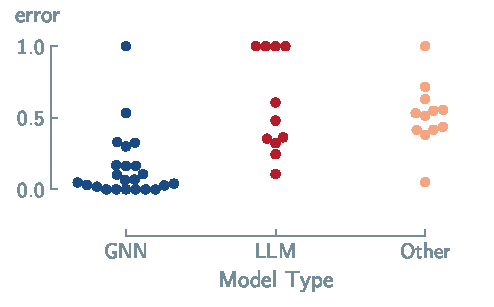
\includegraphics{figures/property_mattext.pdf}
    \caption{\textbf{Normalized error distributions for materials property prediction models across different architectures}. Each point represents the normalized error of a model on a specific property prediction task. Normalization was achieved with min/max values of each dataset to produce a range of errors between 0 and 1. The first column (blue) shows \gls{gnn} based models, the second column (red) displays \gls{llm} approaches, and the third column (orange) represents other baseline methods and \gls{sota} models, including \modelname{CrabNet}. \autocite{Wang_2021} Lower values indicate better predictive performance. Data adapted from \textcite{alampara2024mattext}}
    \label{fig:property_limitations}
\end{figure}


In the revised version, we have now additionally consolidated and carefully added known \textbf{Limitations} and \textbf{Open Challenges} into separate subsections in each of our application sections.  These sections are intended to make readers aware that, despite the existing work, \glspl{gpm}, and especially \glspl{llm}, still face significant problems for many tasks, such as property prediction. For example, in the section of the figure above (section 6.1) we added the following limitations and open challenges section.

\begin{quote}
    

\paragraph{Limitations}

A significant challenge for \glspl{gpm} in chemistry lies in managing dataset limitations and selecting appropriate chemical representations. Practical applications often suffer from highly unbalanced datasets, where examples of optimal materials are vastly outnumbered by poor-performing ones, forcing difficult compromises that can diminish model performance \autocite{vanherck2025assessment}. The choice of how a material is represented (\gls{smiles} notation versus \gls{iupac}) also critically impacts performance, indicating that data preprocessing remains a crucial consideration.

Beyond data issues, architectural constraints present another barrier as illustrated in \Cref{fig:property_limitations}. \textcite{alampara2024mattext} reveal that while \glspl{llm} are effective for tasks relying on compositional information, they struggle to interpret geometric or spatial data when it is encoded in text. This suggests a fundamental limitation of transformer-based architectures for applications requiring spatial reasoning. Consequently, the conventional assumption that performance can be universally improved by scaling up model size or pre-training data is challenged \autocite{frey2023neural}. Such scaling may not overcome the inherent bias against geometric understanding.

\paragraph{Open Challenges}
\begin{itemize}
    \item \textbf{Encoding 3D Structure}: Developing methods to effectively represent and integrate geometric, spatial, and structural information to overcome their inherent bias toward compositional data.
    \item \textbf{Dynamic Knowledge Integration}: Move beyond static fine-tuning to establish a reliable, real-time framework that can incorporate new, evolving scientific findings without catastrophic forgetting.
    \item \textbf{Fundamental Architectural Shifts}: Exploring whether many of the existing \gls{gpm} architectures are sufficient or if new, specialized ones are needed to capture complex relationships in molecular and materials science.
\end{itemize}

\end{quote}

\end{reply}

\begin{point}
Related to above, there is little mention of how LLMs might be misled—by improper RAG, low-quality fine-tuning datasets, or naively designed tasks. E.g. user looking for a material, RAG gives an out-dated or retracted article and LLM becomes confident in its answer it because the way RAG works. or user intentionally prompts or fine-tune in a way the output can be controlled so they end up with good looking scores. Some discussion around the risks. Are there best practices for validation when using these models in the wild? This would help readers adopt the tools responsibly.
\end{point}

\begin{reply}
Following this suggestion, we now discuss the problems with RAG in Section 5.3.3, where we state in the limitations section:
\begin{quote}
\Glspl{llm} and \gls{llm}-based systems are valuable information-gathering tools, but they have critical limitations. Their knowledge becomes outdated immediately after training. Without additional tools, they cannot identify when retrieved sources have been retracted or corrected. 

Effective knowledge gathering requires human-\gls{ai} collaboration. Current systems struggle to ask relevant clarifying questions.\autocite{choudhury2025bed0llm0} Domain-specific benchmarks for evaluating this capability remain absent, hindering progress in developing truly interactive knowledge-gathering agents.
\end{quote}

and in the 5.3.4 section, the open challenges read

\begin{quote}
\begin{itemize}
    \item \textbf{Multimodal Understanding.} Current models cannot reliably extract data from plots, tables, and figures.\autocite{alampara2024probing,gupta2022discomat0} This severely limits data extraction because substantial chemical knowledge exists only in visual formats. Improved multimodal capabilities are essential for comprehensive literature mining.
    
    \item \textbf{Source Quality Assessment.} Citation counts and journal impact factors provide crude quality signals. How to select high-quality sources. Scholarly metrics alone are insufficient.
\end{itemize}

\end{quote}

This discussion addresses the risks of using RAG with outdated or retracted sources, as well as other potential failure modes.

Towards the general best practices for validation, we have now added an example box summarizing some of the principles in the design of the evaluation section (section 4.2), see below:

\begin{examplebox}[label={example:best_practices}]{Best practices for robust model evaluation}
\textbf{Setup and Reporting}
\begin{itemize}
    \item Ensure full reproducibility: document all steps from data preparation to scoring.
    \item Fix and report: model checkpoint or \gls{api} version, date and time, inference settings (e.g., temperature, context length).
    \item Store all evaluation assets (prompts, datasets, scripts) under version control for traceability.
    \item Clearly define: evaluation goal, task scope, data origin, and underlying assumptions.
\end{itemize}

\textbf{Validation and Sanity Checks}
\begin{itemize}
    \item Check for potential training data leakage by testing partial completions or measuring accuracy drop under paraphrasing \autocite{duarte2024detecting}.
    \item Use clear-cut factual questions phrased in multiple ways to test consistency.
    \item Include prompts containing obvious errors (e.g., “benzene is not aromatic”) to probe factual robustness.
    \item Perform repeated runs with different random seeds or sampling temperatures to estimate uncertainty.
\end{itemize}


\textbf{Bias and Construct Validity}
\begin{itemize}
    \item Verify that tasks measure intended skills (reasoning vs. recall).
    \item Balance question difficulty; include control and counterfactual items.
    \item Check dataset composition for chemical space or label bias.
\end{itemize}

\textbf{Publication and Communication}
\begin{itemize}
    \item Double-check factual claims against trusted references.
    \item Report both metrics and qualitative error patterns.
    \item Use structured evaluation cards \autocite{alampara2025lessons} for transparency.
\end{itemize}
\end{examplebox}




\end{reply}

\begin{point}
A controversial topic: how much do GPMs really understand chemistry? Do they need to understand chemistry in order to be good at outputting chemistry answers? If yes, how can they be improved? If no, how to learn real insights from benchmarking?
\end{point}

\begin{reply}
 We have now added some discussion about it in Section 8 (Outlook and Conclusions). Which now reads,

\begin{quote}
    It remains unclear whether generative models achieve a genuine understanding of chemistry or merely excel at pattern recognition, a distinction obscured by the lack of methods to quantify chemical reasoning \autocite{alampara2024probing}. This uncertainty challenges the need for human-interpretable output, implying that the latent knowledge within hidden embeddings may be more significant \autocite{hao2024training}.
\end{quote}

Additionally, we also added a paragraph in the same section discussing when to use a \gls{gpm}. It reads:

\begin{quote}
    With all this flexibility, it becomes tempting to deploy \glspl{gpm} across a wide range of problems in the chemical sciences. However, as discussed in the previous sections, they are not always a direct replacement for existing approaches. In some cases, using a \gls{gpm} may be unnecessary and inefficient. That said, there are clear scenarios where \glspl{gpm} offers distinct advantages. When data is unstructured or \enquote{fuzzy}---such as text-based descriptions or incomplete experimental records lacking explicit molecular structures---\glspl{gpm}, become valuable alternatives where specialized pipelines like \glspl{gnn} would be inapplicable. Similarly, in extremely low-data regimes where specialized pipelines or domain-specific foundation models would overfit, \gls{gpm} embeddings can provide more robust predictions than random baselines. Finally, for dynamic environments that require iterative reasoning, interpretation, and adjustment of the system states, \gls{gpm}-powered agents are well-suited. In contrast, when clean datasets are available and inductive biases are well-understood, domain-specific models typically offer superior performance and interpretability.
\end{quote}


We would also like to highlight that we had some meta-analysis showing the performance comparison across different model architectures. For example, \Cref{fig:property_limitations} 

\end{reply}

\begin{point}
One area that I think deserves more attention is databases. Section 2 and Table 6 touch on data creation, but for foundation models the quality and diversity of pretraining data is central. Are there enough large-scale, clean chemical datasets for pre/post training? What about coverage of underexplored materials or experimental data? What percentage are simulated data / measurement data? This is a practical bottleneck that's worth calling out more directly.
\end{point}

\begin{reply}

We have now added some general discussion at the end of Section 2 about the lack of data quantitatively, but also qualitatively (e.g., negative experiments data is still missing) to illustrate that the available data to train such models is orders of magnitude smaller than the ideal amount of data needed and that it is already out there for other scientific domains such as math. The text now states:

\begin{quote}
    Future Directions

    A primary obstacle in the development of \glspl{gpm} for chemistry is the immense scale of data required for pre-training, which reaches into the trillions of tokens. This demand is illustrated by models like \modelname{Llama 3}, trained on 15 trillion tokens. Yet the largest open-source chemistry corpus available contains only approximately 75 billion tokens.\autocite{mirza2025chempile0} 
    Beyond its insufficient volume, this dataset is constrained by restrictive licenses and is not ideally suited for the primary pre-training phase. Furthermore, existing data resources lack documentation of negative or failed experiments and reasoning data related to routine laboratory tasks. The absence of such data impedes the development of robust chemistry problem-solving and planning capabilities in \glspl{gpm}. 
    This situation stands in contrast to fields like mathematics, where initiatives such as DeepSeek have successfully leveraged large, domain-specific datasets---for instance, 120 billion math tokens---for continual pre-training \autocite{shao2024deepseekmath0}.
    
    Despite the apparent difficulty of amassing diverse data on this scale, we contend that this challenge is accessible through a coordinated community effort. 
\end{quote}

In addition, for some application sections where data is a limiting factor, we added comments in the new \textbf{Limitations} and \textbf{Open Challenges} sections. For instance, in the Retrosynthesis section, we now include in the limitations:

\begin{quote}
    \glspl{gpm} inherit the fundamental constraints associated with domain-specific models for retrosynthesis, which primarily concern data and evaluation methodologies. The prevailing reliance on patent-derived data introduces a significant bias, as these datasets are dominated by a limited set of reaction types and predominantly feature single-step examples. Furthermore, the absence of negative results and the frequent omission of experimental conditions can mislead model training \autocite{Lee2024noise, Voinarovska2023when, Saebi2023onthe, Maloney2023negative, Tadanki2025dissecting}. The evaluation paradigms suffer from a parallel shortcoming, as they are largely designed for single-step routes and fail to adequately capture the complexities of real-world, multi-step case studies \autocite{TorrenPeraire2024models, maziarz2025re, liu2024evaluating}.

    A further significant challenge, exacerbated in the context of \glspl{gpm}, is data leakage. The vast scale of data used for training these models often leads to saturated benchmarks, where high performance may reflect memorization rather than genuine generalization.
\end{quote}

Similarly, one of the open Challenges of this section states:

\begin{quote}
    \textbf{Data Quality and Bias}: To build more robust and generalizable models, the field must integrate higher-quality data from peer-reviewed scientific literature. This requires the development of standardized extraction schemas and data cleaning protocols to create a balanced and reliable training corpus \autocite{rios2025llm, mehr2020universal}.
\end{quote}

\end{reply}

\begin{point}
The figures are visually appealing and help organize the concepts. That said, some are too generic. Many look like a perspective-style sketch rather than a reference figure. Consider adding more concrete visual examples of inputs, outputs, or workflows from real models—especially for readers newer to GPMs. I like some figures do give some simple examples that can be very helpful, but some others seem to be beneficial from more details than just some icons.
\end{point}

\begin{reply}
We have now reviewed the figures, removing some of them that we considered non-helpful in Sections 5.8 and 7.1 (e.g., old Figure 23 in the education section, which was icon-heavy and did not provide additional information). In addition, we added a figure with a more specific chemical example in Section 5.5 to provide readers with more concrete visual examples of inputs, outputs, and workflows.
\end{reply}

\begin{point}
I also think a short paragraph somewhere (Section 7 probably?) on the resource cost of \glspl{gpm} would be a good addition. Fine-tuning or even training large parameter model isn't trivial. For groups used to training conventional ML models or doing DFT, the compute and environmental footprint of these models may be surprising. A short comparison table or rough estimate would be useful for context.
\end{point}

\begin{reply}

We have now added the cost in terms of both time, data and energy in the model adaptation table in section 3.11 (see \Cref{tab:model_adaptation})

\begin{table}[H]
    \centering
    \caption{\textbf{Model Adaptation Approaches Overview:} This table provides a rough overview of the estimated time, data, required \gls{ml} knowledge and estimated energy cost for each approach. Each method (listed in the first column) is paired with an approximate implementation time, the estimated dataset size, the level of \gls{ml} expertise needed and estimated energy cost.  These estimates assume that you have at least a bachelor's level of understanding of chemistry and at least some computational background. The energy costs are estimated by simulations \cite{ozcan2025quantifying, luccioni2024light} accounting for the number of model calls, architecture, model size and input length.}
\begin{tabular}{lllll}
\toprule
    \textbf{Model adaptation}  & \textbf{Time}    & \textbf{Data}   & \textbf{ML knowledge} & 
    \textbf{Energy Cost} \\ 
\midrule
Pre-training       & Weeks   & 1M--1B+      & Very High & 50MWh - 1GWh  \\
Zero-shot prompting & Minutes & None        & None & \textless 10Wh \\
Few-shot Prompting   & Hours   & \textless 10 & None  & \textless 1kWh  \\
Fine-tuning         & Days    & \textless 10k         & High     &   100kWh - 50MWh  \\
\toprule
    \textbf{Coupling into systems} \\ 
\midrule
RAG                & Days    & 100k--1M+    & Low     &   \textless 1kWh   \\
Tool-Augmentation   & Days    & None / 10k+ & Low     &  \textless 1kWh  \\
\bottomrule
\end{tabular}
    \label{tab:model_adaptation}
\end{table}

\end{reply}


\begin{point}
In the introduction section, it says GPMs can ``easily adapt to new settings'' (Section 1), which I think is overly optimistic. While some foundational models can do a better job in transfer to knowledge, the word ``easily'' should probably be avoided here—it depends heavily on the task, the model, and the available data.
\end{point}

\begin{reply}
We have now addressed this by rewriting the section, which now reads:
\begin{quote}
A \gls{gpm} is a model that has been pre‑trained on a broad, heterogeneous corpus spanning multiple data modalities (text, images, graphs) or representations (e.g., common names, 3D coordinates, molecular images).
It can be applied to a wide spectrum of downstream tasks that differ in objective (classification, regression, generation, reasoning), input format, and domain---ranging from natural‑language processing to chemistry and vision---with little or no task‑specific fine‑tuning.
A \gls{gpm} supports zero‑shot, few‑shot, or transfer learning and can serve as the core component of autonomous agents.
\end{quote}

 We also added Table 1 (see \Cref{tab:gpm}) to differentiate \glspl{gpm} from other models:
\end{reply}

\begin{point}
There are a few exciting recent developments not mentioned, particularly those combining LLMs with knowledge graphs for scientific reasoning. Also, I've seen several examples in 2023–2025 of LLM+agent systems being used for real lab explorations. I'd also love to see more discussion to reasoning LLMs. ether0 is mentioned. the architecture and implications of reasoning-focused models for chemical task will be interesting to readers.
\end{point}

\begin{reply}
We have now improved the discussion about reasoning models by expanding our discussion of reasoning-focused architectures in section 5.2 (Existing \glspl{gpm} for Chemical Science). 
We expanded the paragraph on Reasoning-Based Approaches, which now reads:

\begin{quote}
    
\paragraph{Reasoning-Based Approaches} A recent development in chemical \glspl{gpm} incorporates explicit reasoning capabilities. The \modelname{ether0} model demonstrated this approach as a 24 billion-parameter reasoning model trained on over 640k chemically-verifiable problems (e.g., through code) across 375 tasks, including single-step retrosynthesis, molecular editing, and reaction prediction \autocite{narayanan2025training}. 
Unlike previous models, \modelname{ether0}'s training used a novel \gls{rl} approach. First, \modelname{DeepSeek-R1} was prompted to create long \gls{cot} traces ending in a \gls{smiles}. These traces were used to fine-tune a pre-trained \modelname{Mistral-Small-24B} using \gls{sft}, resulting in a \enquote{base reasoner} model. This model underwent \gls{rl} using \gls{grpo} on several verifiable chemical tasks to create \enquote{specialist} models---one for each task. High-quality outputs from these specialist models were selected and used to fine-tune the \enquote{base reasoner} to create a \enquote{generalist} model, capable of reasoning about all the tasks. In the last step, the generalist model undergoes another round of \gls{rl} on the chemical tasks to improve the performance. This method shows that structured problem-solving approaches can significantly improve performance on complex chemical tasks without the need for massive domain-specific corpora. 
\end{quote}

In the Post-Supervised Adaptation section (section 3.7), we added a worked-out example showing the plausibility of reasoning models for optimizing properties, aiming to motivate readers to explore reasoning-based models (shown below):

\begin{examplebox}[label={example:rl}]{Optimizing solar cells}

\textbf{Goal:} Design perovskites that are both stable (high thermal/phase stability) and high-performing (optimal bandgap for light absorption).

\textbf{State:} Current partial perovskite formula (e.g., \ce{ABX3} lattice with partial cation/anion substitutions). \\

\textbf{Action:} Substitute the next ion or additive (e.g., replace \ce{A}-site with \ce{Cs+} or add \ce{Cl-} dopant). \\

\textbf{Reward:}
\begin{itemize}
    \item \texttt{+1} for stability (e.g., based on Goldschmidt tolerance factor).
    \item \texttt{+1} for bandgap tuning (\texttt{1.5 to 1.8 eV} ideal for single-junction cells).
    \item \texttt{-1} for defect proneness (e.g., halide migration).
\end{itemize}

\textbf{Episode Example:}

\begin{itemize}
    \item Start with \ce{PbI2} scaffold (\ce{B} and \ce{X} sites) $\rightarrow$ add \ce{MA+} (methylammonium) at \ce{A}-site $\rightarrow$ Reward: \texttt{+0.5} (good initial bandgap but low stability due to organic volatility).
    \item Co-substitute with \ce{Cs+} and \ce{FA+} (formamidinium) $\rightarrow$ Reward: \texttt{+1.7} (improved tolerance factor \textgreater{}\texttt{0.9}, stable mixed-cation perovskite with approx. ~ \texttt{1.6 eV} bandgap).
    \item Over-dope with excess \ce{Br-} $\rightarrow$ Reward: \texttt{-0.7} (widens bandgap too much \textgreater{}\texttt{1.8 eV}, reducing PCE; also increases defects).
\end{itemize}


The model learns to generate perovskite compositions that maximize cumulative reward, naturally discovering stable, high-PCE materials in the vast compositional space for next-gen solar cells. Note, however, that attempting this or a problem would require designing reward functions that can score actions taken by the agent.

\end{examplebox}

However, as this is currently the only reasoning model specifically developed for the chemical sciences, the discussion is necessarily focused on this example.
\end{reply}

\begin{point}
Finally, I think the current manuscript title (while short and impressive) implies the field is already fully developed (especially for chemists who dont have prior knowledge in this area). A slight revision might help. Either modify title or abstract to let readers know this is an evolving topic. Otherwise, the title might suggest a kind of static completeness that doesn't reflect how fast the field is changing.
\end{point}

\begin{reply}
We have updated the title and abstract to better reflect that this is an evolving field. 
The title now reads 
\enquote{General-Purpose Models for the Chemical Sciences:
LLMs and Beyond}. The abstract closes with 
\begin{quote}
    \enquote{While many of
these applications are still in the prototype phase, we expect that the increasing interest
in \glspl{gpm} will make many of them mature in the coming years.}
\end{quote}
\end{reply}
